\documentclass[reqno,10pt]{amsart}
\usepackage[utf8]{inputenc}
\usepackage{a4wide,amsmath,amsfonts,amssymb,amsthm}
\usepackage{tikz}
\usetikzlibrary{math}
\tikzmath{\Num=200;}
\tikzmath{\Numbis=200;}

\begin{document}

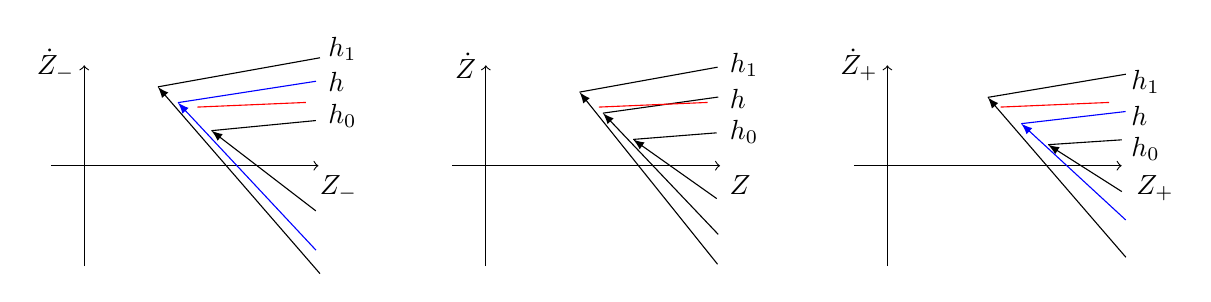
\begin{tikzpicture}[scale=0.85]
        %%%% axis
        \draw[->,,samples=\Num] (-8,0) -- (-4,0);
        \draw[->,samples=\Num] (-7.5,-1.5) -- (-7.5,1.5);
        \draw (-3.7,0) node[below] {$Z_-$};
        \draw (-7.5,1.5) node[left] {$\dot{Z}_-$};

        %%% three solutions of the phase portrait
        \draw [->,>=latex,domain=-1.6:1,samples=\Num] plot [variable=\t] (-6.6+\t*\t,{rad(atan(\t))/1.5});
        \draw [domain=1:1.6,samples=\Num] plot [variable=\t] (-6.6+\t*\t,{rad(atan(\t))/1.5});
        \draw (-4,0.75) node[right] {$h_0$};

        \draw [->,blue,>=latex,domain=-1.75:1,samples=\Num] plot [variable=\t] (-7.1+\t*\t,{rad(atan(\t))*1.2});
        \draw [blue,domain=1:1.75,samples=\Num] plot [variable=\t] (-7.1+\t*\t,{rad(atan(\t))*1.2});
        \draw (-4,1.25) node[right] {$h$};

        \draw [->,>=latex,domain=-1.85:1,samples=\Num] plot [variable=\t] (-7.4+\t*\t,{rad(atan(\t))*1.5});
        \draw [domain=1:1.85,samples=\Num] plot [variable=\t] (-7.4+\t*\t,{rad(atan(\t))*1.5});
        \draw (-4,1.75) node[right] {$h_1$};

        \draw [red,domain=1.2:1.75,samples=\Num] plot [variable=\t] (-7.25+\t*\t,{rad(atan(\t))*(1+\t *sin(\t*1200)/15});


    %%% middle picture : comparison with Z
        %%%% axis
        \draw[->,samples=\Num] (-2,0) -- (2,0);
        \draw[->,samples=\Num] (-1.5,-1.5) -- (-1.5,1.5);
        \draw (2.3,0) node[below] {$Z$};
        \draw (-1.5,1.5) node[left] {$\dot{Z}$};

        %%% three solutions of the phase portrait
        \draw [->,>=latex,domain=-1.5:1,samples=\Num] plot [variable=\t] (-0.3+\t*\t,{rad(atan(\t))/2});
        \draw [domain=1:1.5,samples=\Num] plot [variable=\t] (-0.3+\t*\t,{rad(atan(\t))/2});
        \draw (2,0.5) node[right] {$h_0$};

        \draw [->,>=latex,domain=-1.65:1,samples=\Num] plot [variable=\t] (-0.75+\t*\t,{rad(atan(\t))});
        \draw [domain=1:1.65,samples=\Num] plot [variable=\t] (-0.75+\t*\t,{rad(atan(\t))});
        \draw (2,1) node[right] {$h$};

        \draw [->,>=latex,domain=-1.75:1,samples=\Num] plot [variable=\t] (-1.1+\t*\t,{rad(atan(\t))*1.4});
        \draw [domain=1:1.75,samples=\Num] plot [variable=\t] (-1.1+\t*\t,{rad(atan(\t))*1.4});
        \draw (2,1.5) node[right] {$h_1$};

        \draw [red,domain=1.2:1.75,samples=\Num] plot [variable=\t] (-1.25+\t*\t,{rad(atan(\t))*(1+\t *sin(\t*1200)/15});

    %%%% axis
        \draw[->,samples=\Num] (4,0) -- (8,0);
        \draw[->,samples=\Num] (4.5,-1.5) -- (4.5,1.5);
        \draw (8.5,0) node[below] {$Z_+$};
        \draw (4.5,1.5) node[left] {$\dot{Z}_+$};

        %%% three solutions of the phase portrait
        \draw [->,>=latex,domain=-1.45:1,samples=\Num] plot [variable=\t] (5.9+\t*\t,{rad(atan(\t))/2.5});
        \draw [domain=1:1.45,samples=\Num] plot [variable=\t] (5.9+\t*\t,{rad(atan(\t))/2.5});
        \draw (8,0.25) node[right] {$h_0$};

        \draw [->,blue,>=latex,domain=-1.6:1,samples=\Num] plot [variable=\t] (5.5+\t*\t,{rad(atan(\t))*0.8});
        \draw [blue,domain=1:1.6,samples=\Num] plot [variable=\t] (5.5+\t*\t,{rad(atan(\t))*0.8});
        \draw (8,0.75) node[right] {$h$};

        \draw [->,>=latex,domain=-1.75:1,samples=\Num] plot [variable=\t] (5+\t*\t,{rad(atan(\t))*1.3});
        \draw [domain=1:1.75,samples=\Num] plot [variable=\t] (5+\t*\t,{rad(atan(\t))*1.3});
        \draw (8,1.25) node[right] {$h_1$};

        \draw [red,domain=1.2:1.75,samples=\Num] plot [variable=\t] (4.75+\t*\t,{rad(atan(\t))*(1+\t *sin(\t*1200)/15});

\end{tikzpicture}

\end{document}